% Step-by-step derivation of the structure-parameter and DM uncertainties for SHRINE
% (Sutinjo et al. 2023, S23; ApJ 954, 37). "S23 Eq. N" uses the published numbering (Eqs. 1-20).
\documentclass[11pt]{article}
\usepackage[a4paper,margin=2.3cm]{geometry}
\usepackage{amsmath,amssymb,bm,booktabs,graphicx}
\usepackage{microtype}
\usepackage[hidelinks]{hyperref}
\emergencystretch=1em
\setlength{\parskip}{4pt}
\renewcommand{\labelitemi}{$\bullet$}
\newcommand{\vb}[1]{\boldsymbol{#1}}
\newcommand{\Dn}{\vb D_1}
\newcommand{\Sm}{\vb S}
\newcommand{\ti}{\tilde{\vb i}}
\newcommand{\Di}{\vb\Delta_{\vb i}}
\newcommand{\ah}{\hat{\vb a}}
\newcommand{\nrm}[1]{\lVert #1\rVert}
\newcommand{\na}{\nrm{\vb a}}
\newcommand{\Sc}{\mathcal S}
\newcommand{\ep}{e_\parallel}
\newcommand{\eperp}{\vb e_\perp}
\newcommand{\tch}{\tau_{\nu}}
\newcommand{\xch}{x_{\nu}}
\newcommand{\sch}{\sigma_{\nu}}
\newcommand{\Var}{\operatorname{Var}}
\newcommand{\Cov}{\operatorname{Cov}}
\newcommand{\std}{\operatorname{std}}
\newcommand{\vis}{\textit{Visualisation only (not a derivation step).}\ }

\title{SHRINE uncertainties: step-by-step derivation of the\\ structure-parameter and DM errors}
\author{}
\date{}
\begin{document}
\maketitle
\vspace{-1.5cm}

\section*{Setup and notation}

S23 is Sutinjo et al.\ (2023, ApJ 954, 37); ``S23 Eq.~$N$'' uses the published numbering.

\begin{itemize}
\item At one trial DM $d$ the dedispersed intensity is $\vb i$ ($N$ samples). Its true parts are
$\vb i=\vb s+\vb n$: $\vb s$ is the noiseless burst and $\vb n$ is noise with
$\langle\vb n\rangle=0$ and $\Cov(\vb n)=\langle\vb n\vb n^{T}\rangle$.
\item $\langle\cdot\rangle$ is the average over noise realisations: the same burst at the same DM, with new noise.
\item $\Sm$ is the smoothing matrix (symmetric) and $\Dn$ the $(N-1)\times N$ first difference,
$(\Dn\vb x)_j=x_{j+1}-x_j$ (S23 Eq.~2).
\item $\Sm=\vb C\,{\rm diag}[f(k)]\,\vb C^{T}$ (S23 Eq.~15), with $\vb C$ the orthonormal DCT-II matrix and $f(k)$ S23's
Butterworth response (Eq.~16) with cutoff $k_c$ and order $O$. ${\rm eig}_k$ (S23 Eq.~14) are the eigenvalues of
$\Dn^{T}\Dn$. SHRINE's \texttt{get\_kc} places $k_c$ where the burst's DCT spectrum falls to the noise level.
\item The structure parameter is $\Sc=\nrm{\Dn\Sm\vb i}$, the norm of S23 Eq.~3.
\item S23 Eq.~4 splits the data as $\vb i=\ti+\Di$ with $\ti=\Sm\vb i$ and $\Di=\vb i-\Sm\vb i$. These are
\emph{estimates} of signal and noise built with $\Sm$. Substituting the true parts $\vb i=\vb s+\vb n$,
\begin{equation}
\ti=\Sm\vb s+\Sm\vb n,\qquad \Di=(\vb s-\Sm\vb s)+(\vb n-\Sm\vb n).
\label{eq:split}
\end{equation}
Neither part is pure. $\ti$ contains the in-band noise $\Sm\vb n$ that smoothing cannot remove. $\Di$ contains the
noise that smoothing removed, $\vb n-\Sm\vb n$, and also the burst structure that smoothing removed,
$\vb s-\Sm\vb s$: the \emph{leakage} term. The leakage is the same in every realisation, so it is not noise, but S23
treat all of $\Di$ as noise.
\end{itemize}

\section*{Step 1: split the structure parameter by the true parts}

Define
\begin{equation}
\vb a=\Dn\Sm\vb s,\qquad \vb e=\Dn\Sm\vb n,\qquad \ah=\vb a/\na .
\end{equation}
Then $\Dn\Sm\vb i=\vb a+\vb e$ exactly, so $\Sc=\nrm{\vb a+\vb e}$. $\vb a$ is fixed (it depends only on the
burst); $\vb e$ is random with zero mean.

$\vb s$ and $\vb n$ are not known in practice. The split is still what tells us which statistic is the correct
error; Step~4 replaces the unknowns by estimates.

\section*{Step 2: only the noise along $\vb a$ matters at first order}

Split the noise into a part along $\ah$ and a part perpendicular to it:
\begin{equation}
\vb e=\ep\,\ah+\eperp,\qquad \ep=\ah^{T}\vb e .
\end{equation}
$\ep$ is a signed scalar. Because $\eperp\perp\ah$, Pythagoras gives
\begin{equation}
\nrm{\vb a+\vb e}^{2}=(\na+\ep)^{2}+\nrm{\eperp}^{2}.
\end{equation}
For $\nrm{\eperp}\ll\na$, $\sqrt{X^{2}+Y^{2}}\simeq X+Y^{2}/2X$. Replacing $\na+\ep$ by $\na$ in the last term
changes it only at third order, so to second order in the noise
\begin{equation}
\boxed{\;\Sc\simeq\na+\ep+\frac{\nrm{\eperp}^{2}}{2\na}\;}
\label{eq:S}
\end{equation}
\begin{itemize}
\item $\ep$ is the only noise term at first order. It sets the $1\sigma$ scatter of $\Sc$.
\item $\nrm{\eperp}^{2}/2\na\ge0$ is a second-order positive bias, not an uncertainty.
\item S23's bounds (Eq.~8) are triangle inequalities. They are reached only when the added vector is
parallel to the structure vector (here $\eperp=0$, all of the noise along $\ah$). They are bounds, not $1\sigma$ errors.
\end{itemize}

\begin{figure}[h]
\centering
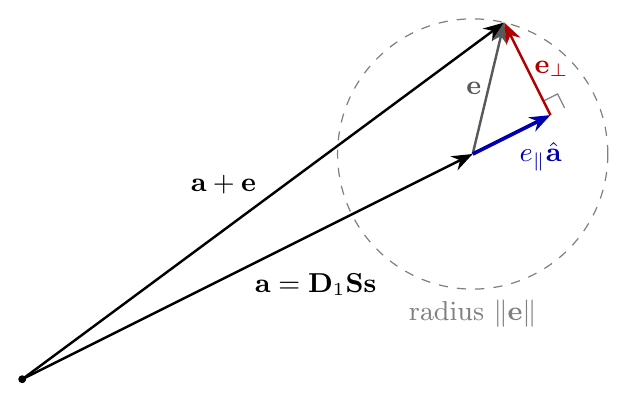
\includegraphics[width=0.55\textwidth]{fig_parallel.png}
\caption{\vis The noise $\vb e$ added to $\vb a$, split into $\ep\ah$ and $\eperp$. Only $\ep$ changes
the length at first order; $\eperp$ tilts the vector. The dashed circle has radius $\nrm{\vb e}$.}
\label{fig:par}
\end{figure}

\section*{Step 3: variance of $\ep$}

\paragraph{3a. Weights.}
$\ep=\ah^{T}\Dn\Sm\vb n$. Define the row of weights
\begin{equation}
\vb w=\ah^{T}\Dn\Sm\qquad(1\times N),\qquad\text{so}\qquad \ep=\vb w\vb n=\sum_t w_t n_t .
\end{equation}
$w_t$ is the first-order change of $\Sc$ per unit change of noise sample $n_t$. It is fixed by the burst.

\paragraph{3b. Mean.}
Each $w_t$ is a constant and each $n_t$ is one value of the vector $\vb n$. If $\langle n_t\rangle=0$, then
$\langle\ep\rangle=\sum_tw_t\langle n_t\rangle=0$. (A constant offset in $\vb n$ is removed by $\Dn$ anyway.)

\paragraph{3c. Variance.}
With zero mean, $\Var(X)=\langle X^{2}\rangle-\langle X\rangle^{2}=\langle X^{2}\rangle$, so $\sigma^{2}=\langle\ep^{2}\rangle$.
Write the square as the sum times itself, counting the second copy with its own dummy label $t'$ so that
every term of one copy multiplies every term of the other:
\begin{equation}
\sigma^{2}=\Big\langle\Big(\sum_tw_tn_t\Big)\Big(\sum_{t'}w_{t'}n_{t'}\Big)\Big\rangle
=\sum_t\sum_{t'}w_tw_{t'}\langle n_tn_{t'}\rangle=\vb w\,\Cov(\vb n)\,\vb w^{T}.
\end{equation}
$\langle n_tn_{t'}\rangle$ is element $(t,t')$ of $\Cov(\vb n)$. Its diagonal ($t'=t$) is the variance $\sigma_t^{2}$.

\paragraph{3d. Noise uncorrelated between samples.}
$\langle n_tn_{t'}\rangle=\sigma_t^{2}$ if $t'=t$ and $0$ otherwise, so the $t'$ sum keeps one term,
$\sum_{t'}w_{t'}\langle n_tn_{t'}\rangle=w_t\sigma_t^{2}$, and
\begin{equation}
\boxed{\;\sigma^{2}=\sum_tw_t^{2}\sigma_t^{2}\;}
\label{eq:sig}
\end{equation}
For white noise, $\sigma^{2}=\sigma_n^{2}\sum_tw_t^{2}$. $\sigma$ is the $1\sigma$ uncertainty of $\Sc$, and the
relative uncertainty is $\sigma/\Sc$.

\section*{Step 4: evaluating $\sigma$ from the data}

\paragraph{4a. Direction.}
$\ah$ is unknown. Estimate it from the data,
\begin{equation}
\ah\simeq\frac{\Dn\Sm\vb i}{\nrm{\Dn\Sm\vb i}}=\frac{\vb a+\vb e}{\nrm{\vb a+\vb e}} .
\end{equation}
This is tilted from the true $\ah$ by an angle $\theta$ with $\tan\theta=\nrm{\eperp}/(\na+\ep)$, so
$\theta\simeq\nrm{\eperp}/\na$.

\paragraph{4b. Size of $\nrm{\eperp}$.}
For any fixed matrix $\vb M$ and noise uncorrelated between samples,
\begin{equation}
\nrm{\vb M\vb n}^{2}=\sum_j\Big(\sum_tM_{jt}n_t\Big)^{2}=\sum_j\sum_t\sum_{t'}M_{jt}M_{jt'}n_tn_{t'}
\quad\Rightarrow\quad
\langle\nrm{\vb M\vb n}^{2}\rangle=\sum_j\sum_tM_{jt}^{2}\sigma_t^{2},
\label{eq:Mn}
\end{equation}
by the same collapse of the $t'$ sum as in 3d. With $\vb M=\Dn\Sm$ this is $\langle\nrm{\vb e}^{2}\rangle$. Define
\begin{equation}
N_e=\langle\nrm{\vb e}^{2}\rangle/\sigma^{2}:
\end{equation}
the total noise power in $\vb e$ divided by the part along $\ah$ ($\langle\ep^{2}\rangle=\sigma^{2}$), i.e.\ how many
directions' worth of noise $\vb e$ carries. It would be $N-1$ (the length of $\vb e$) for isotropic noise; in our
simulations ($N=2048$, $k_c\simeq40$) $N_e\simeq$ 40--45. Since $\langle\nrm{\eperp}^{2}\rangle=(N_e-1)\sigma^{2}$,
\begin{equation}
\theta\simeq\sqrt{N_e-1}\;\sigma/\na\simeq6\,\sigma/\na .
\end{equation}
The estimated direction is good when $\na\gg6\sigma$. The relative error it introduces in $\sigma$ is of order $\theta$.
In our simulations $\theta\simeq0.2$ at burst amplitude 0.5, and $\sigma$ computed from the data matched the Monte Carlo
to within $\sim$10\%.

\paragraph{4c. Weights.}
$\vb w=\ah^{T}\Dn\Sm$. First $(\ah^{T}\Dn)_t=\hat a_{t-1}-\hat a_t$ (with $\hat a_0=\hat a_N=0$; $\ah$ has $N-1$
entries), then smooth the result with $\Sm$.

\paragraph{4d. Noise level.}
For white noise with standard deviation $\sigma_n$ per sample, take $\sigma_n$ from off-pulse data, or from the on-pulse DCT coefficients above $k=N/4$,
where the burst has no power:
$\hat\sigma_n=1.4826\,{\rm median}_{k>N/4}|(\vb C^{T}\vb i)_k|$ (the orthonormal DCT leaves the white-noise
variance unchanged in every mode). For self-noise, take $\sigma_t^{2}$ as the local mean square of the series
rebuilt from the modes $k>N/4$ only, divided by $3/4$ (the fraction of white-noise variance that
reconstruction keeps). Then use Eq.~(\ref{eq:sig}).

\section*{Step 5: what S23's radius measures (S23 Eqs.~6, 7, 19)}

\paragraph{5a. Split S23's residual.}
Apply $\Dn\Sm$ to $\Di$ from Eq.~(\ref{eq:split}):
\begin{equation}
\Dn\Sm\Di=\vb d_s+\vb d_n,\qquad \vb d_s=\Dn\Sm(\vb s-\Sm\vb s),\qquad \vb d_n=\Dn\Sm(\vb n-\Sm\vb n).
\end{equation}
$\vb d_s$ is the leakage term after $\Dn\Sm$: burst structure that smoothing removed, smoothed again. It is the same in
every realisation, so it is not noise. $\vb d_n$ is random with zero mean.

\paragraph{5b. Expected squared radius.}
The cross term averages to zero, $2\vb d_s^{T}\langle\vb d_n\rangle=0$, so
\begin{equation}
\langle\nrm{\Dn\Sm\Di}^{2}\rangle=\nrm{\vb d_s}^{2}+\langle\nrm{\vb d_n}^{2}\rangle .
\end{equation}
$\vb d_n=(\Dn\Sm-\Dn\Sm\Sm)\,\vb n$ is a fixed matrix times $\vb n$, so $\langle\nrm{\vb d_n}^{2}\rangle$ follows from
Eq.~(\ref{eq:Mn}) with $\vb M=\Dn\Sm-\Dn\Sm\Sm$. It is not zero:
$\langle\vb d_n\rangle=0$, but $\nrm{\vb d_n}^{2}$ is a sum of squares.

\paragraph{5c. Ratio to the true variance.}
Divide by $\sigma^{2}$:
\begin{equation}
\boxed{\;\frac{\langle\nrm{\Dn\Sm\Di}^{2}\rangle}{\sigma^{2}}
=\frac{\langle\nrm{\vb d_n}^{2}\rangle}{\sigma^{2}}\left(1+\frac{\nrm{\vb d_s}^{2}}{\langle\nrm{\vb d_n}^{2}\rangle}\right)\;}
\label{eq:ratio}
\end{equation}
\begin{itemize}
\item \emph{First factor: noise in all directions instead of along $\ah$.} It equals
$N_e\,\langle\nrm{\vb d_n}^{2}\rangle/\langle\nrm{\vb e}^{2}\rangle$. $\vb e=\Dn\Sm\vb n$ is the derivative of the
smoothed noise. $\vb d_n=\Dn\Sm(\vb n-\Sm\vb n)$ is the derivative of the smoothed version of the noise that
smoothing removed, and smoothing it again removes most of it. Per DCT mode $k$ (S23 Eq.~17), $\Dn\Sm$
multiplies by ${\rm eig}_k^{1/2}f(k)$ and $\Dn\Sm-\Dn\Sm\Sm$ by ${\rm eig}_k^{1/2}f(k)[1-f(k)]$. Since
$f(1-f)\le1/4$, with the maximum at $k_c$ where the filter passes half ($f=\tfrac12$), only the noise near $k_c$
survives. It would vanish for a brick-wall filter. In our simulations
$\langle\nrm{\vb d_n}^{2}\rangle\simeq\langle\nrm{\vb e}^{2}\rangle/7.7$, so the first factor is (40--45)/7.7 $\simeq$ 5--6.
\item \emph{Second factor: burst leakage.} $\vb d_s$ lies near $k_c$, where \texttt{get\_kc} places the cutoff
at the point where the burst falls to the noise level, so $\nrm{\vb d_s}^{2}\gtrsim\langle\nrm{\vb d_n}^{2}\rangle$.
$\vb d_s$ scales with burst amplitude, so $\nrm{\vb d_s}^{2}/\langle\nrm{\vb d_n}^{2}\rangle\propto({\rm S/N})^{2}$
at fixed $k_c$. In our simulations the second factor is 4.1 and 12.8 for burst amplitudes 0.5 and 1.0 ($k_c=38$, 40).
\end{itemize}

\paragraph{5d. S23's per-sample reading.}
$\nrm{\Dn\Sm\Di}/\sqrt{N-1}$ (text after S23 Eq.~6) assumes the residual is white over $N-1$ samples. It is
concentrated near $k_c$, so this \emph{under}estimates $\sigma$, by a factor 5--10 in our simulations.

\paragraph{5e. Normalisation (S23 Eq.~7).}
A relative uncertainty is the uncertainty of a quantity divided by that same quantity. $\sigma$ (Step~3) is the
scatter of $\Sc=\nrm{\Dn\Sm\vb i}$, the structure parameter that SHRINE reports and maximises over DM, and
$\Sc\simeq\na+\ep$ (Step~2). So the relative uncertainty is $\sigma/\Sc\simeq\sigma/\na$.

S23 divide instead by $\nrm{\Dn\Sm\ti}=\nrm{\Dn\Sm\Sm\vb i}$ (in the code, \texttt{\_uncertainty\_calc} divides by
the norm of \texttt{combined*fL*c}). This comes from S23 Eq.~5, which treats $\Dn\Sm\ti$ as the signal part of
$\Dn\ti$. But $\Dn\Sm\ti$ is the data smoothed twice: its burst part is $\Dn\Sm\Sm\vb s$, not $\vb a=\Dn\Sm\vb s$.
Per DCT mode $k$ (S23 Eq.~17), with $c_k$ the DCT coefficients of $\vb s$,
\begin{equation}
\nrm{\Dn\Sm\vb s}^{2}=\sum_k{\rm eig}_k\,f(k)^{2}c_k^{2},\qquad
\nrm{\Dn\Sm\Sm\vb s}^{2}=\sum_k{\rm eig}_k\,f(k)^{4}c_k^{2}.
\end{equation}
Since $f(k)\le1$, every mode is reduced, so $\nrm{\Dn\Sm\Sm\vb s}<\na$. The loss is largest near $k_c$, where
$f\simeq\tfrac12$ and where the band pass ${\rm eig}_k^{1/2}f(k)$ of the structure parameter peaks (S23 Fig.~2). In
our simulations the double-smoothed norm is 5--6\% below $\na$ at any S/N. It is a fixed bias set by the burst shape
and $k_c$, not noise, so it does not shrink as the S/N rises, and it inflates the relative uncertainty by the same
5--6\%.

\paragraph{5f. Root cause.}
The leakage ($\vb d_s$) and the normalisation both come from treating $\ti$ as the true signal and $\Di$ as the
noise (S23 Eq.~4), when both mix burst and noise (Eq.~\ref{eq:split}).
The first factor of Eq.~(\ref{eq:ratio}) is the separate radius-versus-projection problem of Step~2.

\section*{Step 6: DM uncertainty}

\paragraph{6a. Structure curve.}
At each trial DM $d$, Steps~1--2 give
\begin{equation}
\Sc(d)\simeq\nrm{\vb a(d)}+\ep(d),
\end{equation}
with $\vb a(d)=\Dn\Sm\vb s(d)$ and $\ep(d)$ the noise along $\ah(d)$. The second-order bias varies slowly with $d$
and is dropped. Let $d_0$ be the peak of the noise-free curve $\nrm{\vb a(d)}$. For a burst with the same profile
in every channel this is the true DM. With drift it can differ; that systematic offset is separate and not
covered here.

\paragraph{6b. Expand about $d_0$.}
\begin{align}
\nrm{\vb a(d)}&\simeq\nrm{\vb a(d_0)}+\tfrac12\nrm{\vb a}''(d_0)\,(d-d_0)^{2},\\
\ep(d)&\simeq\ep(d_0)+\ep'(d_0)\,(d-d_0).
\end{align}
The linear term of the first line is absent because $\nrm{\vb a}'(d_0)=0$ at the peak. $\nrm{\vb a}''(d_0)<0$ is the
curvature, the rate at which the slope changes; near its peak any smooth curve is close to a parabola. So
\begin{equation}
\Sc(d)\simeq\nrm{\vb a(d_0)}+\ep(d_0)+\ep'(d_0)\,(d-d_0)+\tfrac12\nrm{\vb a}''(d_0)\,(d-d_0)^{2}.
\end{equation}
The noise value $\ep(d_0)$ lifts the whole curve and does not move the peak. The noise slope $\ep'(d_0)$ tilts
it: $\Sc'(d_0)=\ep'(d_0)\ne0$, so the curve is no longer flat at $d_0$ and the peak moves.

\paragraph{6c. Peak position.}
At the measured peak $\hat d$, $\Sc'(\hat d)=0$:
\begin{equation}
\ep'(d_0)+\nrm{\vb a}''(d_0)\,(\hat d-d_0)=0\quad\Rightarrow\quad \hat d-d_0=-\frac{\ep'(d_0)}{\nrm{\vb a}''(d_0)} .
\end{equation}
$\nrm{\vb a}''(d_0)$ is fixed and $\std(X/K)=\std(X)/|K|$, so
\begin{equation}
\sigma_{\rm DM}=\frac{\std[\ep'(d_0)]}{|\nrm{\vb a}''(d_0)|}.
\label{eq:sdm0}
\end{equation}

\paragraph{6d. $\ep(d)$ in terms of the channel noise.}
From Step~3, $\ep(d)=\sum_tw(t;d)\,n(t;d)$, where $w(t;d)$ is the weight row computed from the burst
dedispersed at $d$ (it changes with $d$ because the dedispersed burst does; it does not depend on the burst
amplitude). Dedispersion gives
\begin{equation}
n(t;d)=\sum_{\nu}\xch(t+d\,\tch),\qquad \tch=K_{\rm DM}\,(\nu^{-2}-\nu_{\rm ref}^{-2})/t_{\rm samp}.
\end{equation}
\begin{itemize}
\item $t$ is the time-sample index; $\xch(t)$ is the raw noise in channel $\nu$ at sample $t$.
\item $K_{\rm DM}\simeq4.149$\,ms\,GHz$^{2}$\,(pc\,cm$^{-3}$)$^{-1}$, so $\tch$ is in samples per pc\,cm$^{-3}$
and $d\,\tch$ (DM times $\tch$) is channel $\nu$'s delay in samples; dedispersion advances the channel by it.
Fractional shifts are applied as FFT phase shifts.
\item $\nu_{\rm ref}$ is a free choice (see 6g).
\end{itemize}
Hence
\begin{equation}
\ep(d)=\sum_{\nu}\sum_tw(t;d)\,\xch(t+d\,\tch).
\end{equation}

\paragraph{6e. Move the shift onto the weights.}
Relabel $t\to t-d\,\tch$ in each channel:
\begin{equation}
\ep(d)=\sum_{\nu}\sum_tw(t-d\,\tch;d)\,\xch(t).
\label{eq:relab}
\end{equation}
The pairs are unchanged; only the counting label moves. With a one-sample shift,
$\sum_tw_tx_{t+1}=\sum_tw_{t-1}x_t=\ldots+w_4x_5+w_5x_6+w_6x_7+\ldots$: the shift moves to the other factor with
the opposite sign. This is exact for circular (FFT) shifts, and otherwise holds up to edge samples where the
weights are $\simeq0$.

Why: $\xch(t)$ no longer depends on $d$. All the $d$-dependence is in the weights, which are smooth (they
have passed through $\Sm$) and can be differentiated. White noise cannot.

\paragraph{6f. Differentiate.}
In each term $\xch(t)$ is a constant factor, so
\begin{equation}
\ep'(d_0)=\sum_{\nu}\sum_tw'_{\nu}(t)\,\xch(t),\qquad
w'_{\nu}(t)=\frac{\partial}{\partial d}\,w(t-d\,\tch;d)\Big|_{d_0}.
\end{equation}
$w'_{\nu}(t)$ is the change, per unit DM, of the weight that multiplies raw noise sample $\xch(t)$. It
changes because the channel slides under the weight row (by $\tch$ samples per unit DM, so differently in
each channel) and because the row itself changes shape as the dedispersed burst changes.

\begin{figure}[h]
\centering
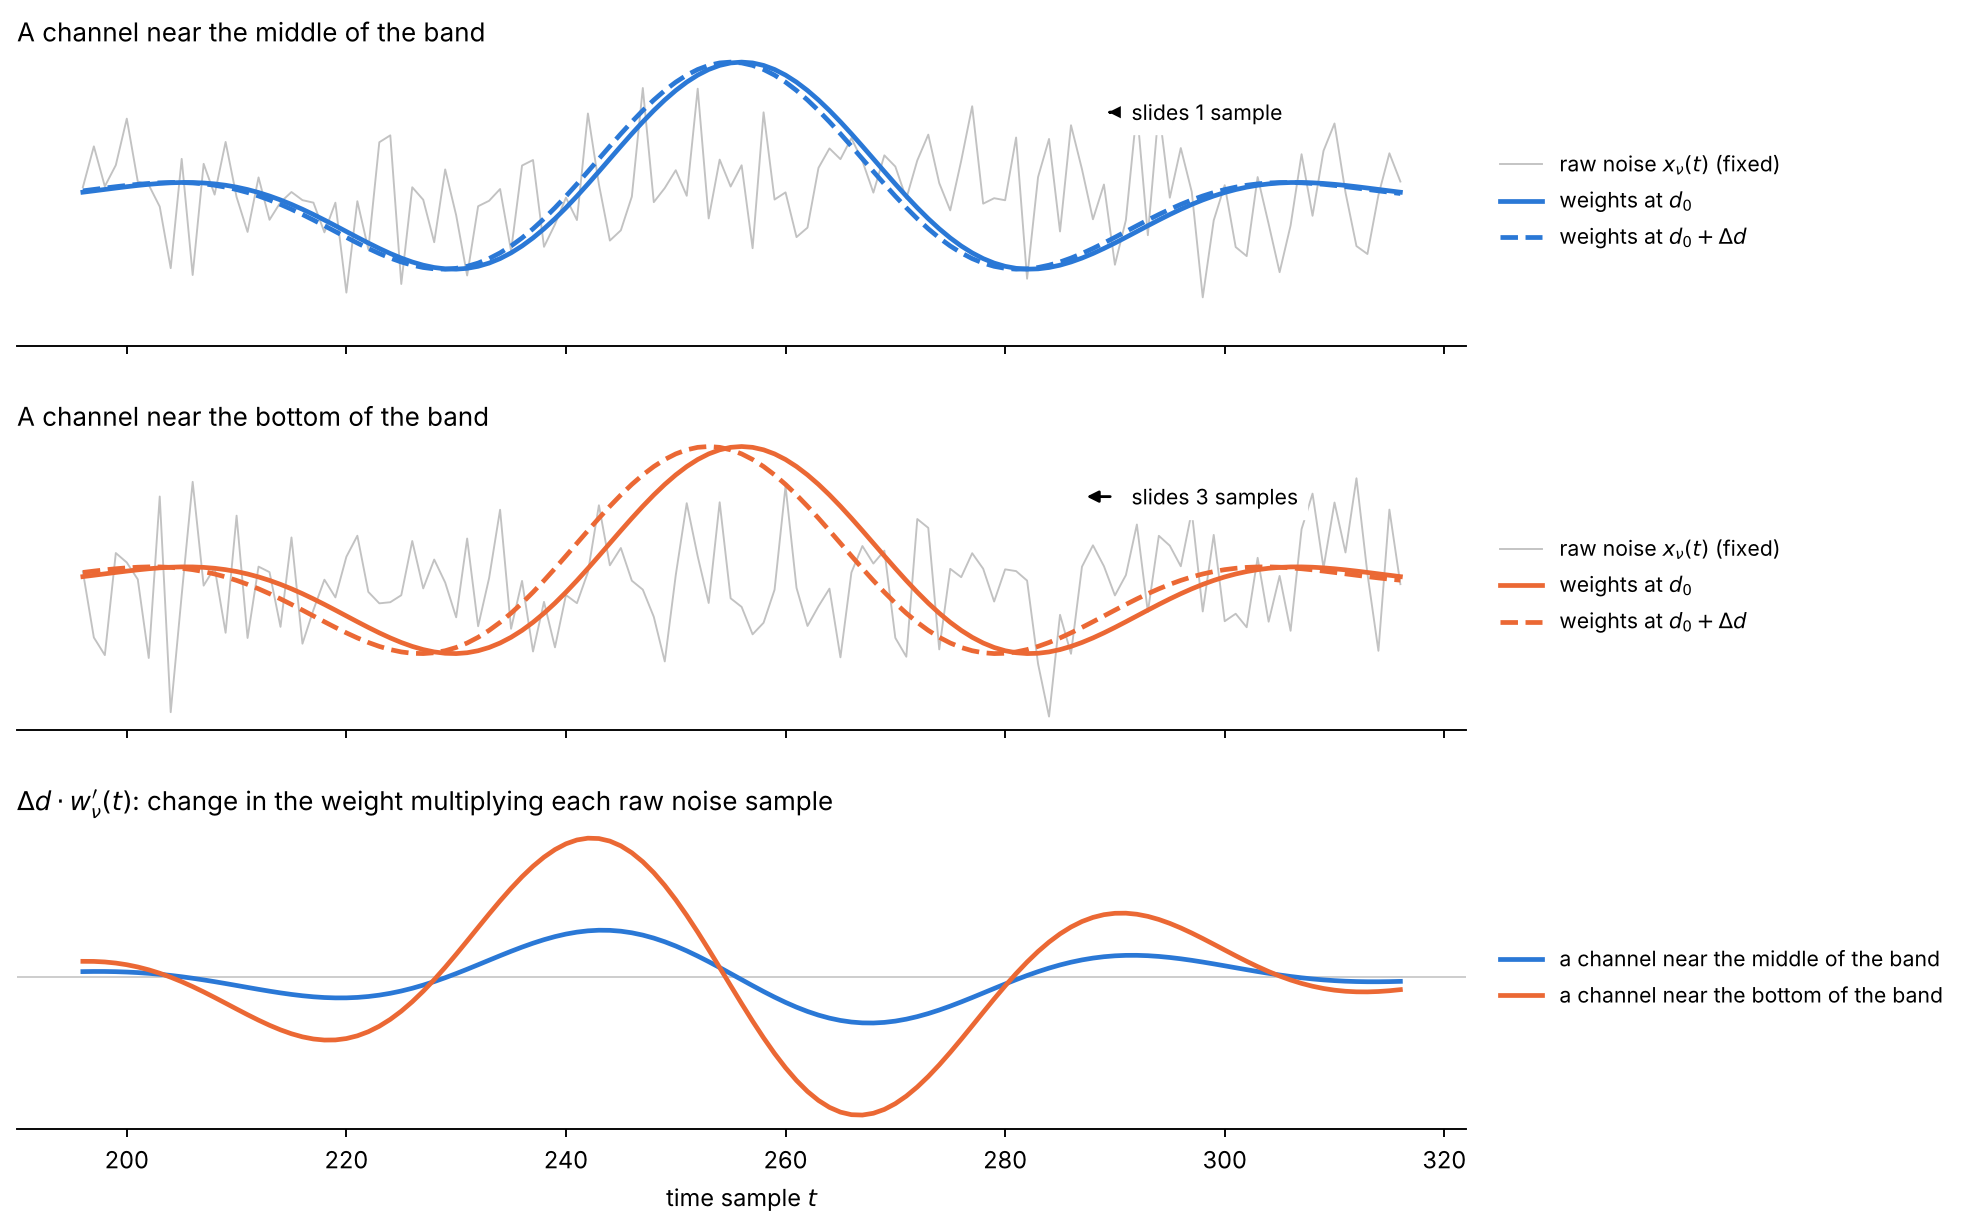
\includegraphics[width=\textwidth]{fig_wprime.png}
\caption{\vis The same weight row over the fixed raw noise of two channels, at $d_0$ (solid) and
$d_0+\Delta d$ (dashed). The two channels slide different distances under the row; the bottom panel is
the resulting change of the weight multiplying each raw noise sample, $\Delta d\cdot w'_{\nu}(t)$. Drawn for a
burst with the same profile in every channel, so the row only slides; with drift or scattering it also
changes shape. Delays are measured from the amplitude-weighted mean delay.}
\label{fig:wp}
\end{figure}

\paragraph{6g. Variance.}
Within one noise realisation, $\xch(t)$ is one dynamic spectrum of noise; $\nu$ and $t$ are summation labels,
$\ep(d)$ is one curve against $d$, and $\ep'(d_0)$ is one number. Across realisations, the burst, the
weights, $w'_{\nu}$, $\tch$ and $d_0$ stay fixed and $\xch(t)$ changes. Assume $\xch(t)$ has zero mean, is
independent between channels and between samples, and has variance $\sch^{2}$. Then, exactly as in Step~3
with the label $(\nu,t)$ in place of $t$: $\langle\ep'(d_0)\rangle=0$, so $\Var=\langle\ep'(d_0)^{2}\rangle$,
and only the terms with $\nu'=\nu$, $t'=t$ survive:
\begin{equation}
\Var[\ep'(d_0)]=\sum_{\nu}\sch^{2}\sum_tw'_{\nu}(t)^{2},
\end{equation}
\begin{equation}
\boxed{\;\sigma_{\rm DM}=\frac{\Big(\sum_{\nu}\sch^{2}\sum_tw'_{\nu}(t)^{2}\Big)^{1/2}}{|\nrm{\vb a}''(d_0)|}\;}
\label{eq:sdm}
\end{equation}
\begin{itemize}
\item $\langle\ep'(d_0)\rangle=0$: to first order $\hat d$ scatters symmetrically about $d_0$.
\item This holds for any burst morphology (drift, scattering, profile evolution).
\item For self-noise, use $\sch(t)^{2}$ inside the $t$ sum.
\item It does not depend on $\nu_{\rm ref}$: changing $\nu_{\rm ref}$ shifts every channel and the weight row
by the same amount, so $w(t-d\,\tch;d)$ is unchanged.
\end{itemize}

\paragraph{6h. Evaluating $\sigma_{\rm DM}$ from the data.}
Everything at $d_0$ is evaluated at the measured peak $\hat d$ (as $\ah$ was in Step~4). None of the following
assumes the same profile in every channel.
\begin{enumerate}
\item \emph{Curvature $\nrm{\vb a}''$.} The measured curve is $\Sc(d)=\nrm{\vb a(d)}+\ep(d)+\ldots$, so its
curvature is the one we want plus noise curvature. Two estimates:
\begin{itemize}
\item \emph{Fit:} least-squares parabola $\Sc(d)\simeq c_0+c_1d+c_2d^{2}$ over the trial DMs with
$|d-\hat d|\le W$; then $\nrm{\vb a}''\simeq2c_2$ (and $\hat d=-c_1/2c_2$).
\item \emph{Finite difference:} $\nrm{\vb a}''\simeq[\Sc(\hat d+h)-2\Sc(\hat d)+\Sc(\hat d-h)]/h^{2}$,
dedispersing at $\hat d\pm h$ if they are not on the grid.
\end{itemize}
$\ep(d)$ is smooth in $d$, so a narrow window or small step also picks up the curvature of the noise, while
too wide a window leaves the region where $\nrm{\vb a(d)}$ is parabolic. Use $W\simeq2$--$3\,\sigma_{\rm DM}$ or
$h\simeq2\,\sigma_{\rm DM}$: start from a guess, compute $\sigma_{\rm DM}$, and refit. In the drifting-burst
test (below) both were unbiased to $\simeq1\%$, with 16--84\% scatter of $\pm$12--15\% at S/N 14 and
$\pm$5--7\% at S/N 38; $W=1.5\,\sigma_{\rm DM}$ or $h=\sigma_{\rm DM}$ increased the scatter by up to a factor of 2.
Check that the result is stable when $W$ or $h$ is changed.
\item \emph{Weight rows.} For each needed $d$, dedisperse the data, set $\ah(d)\simeq\Dn\Sm\vb i(d)/\nrm{\Dn\Sm\vb i(d)}$
and $w(t;d)=\ah(d)^{T}\Dn\Sm$ (Step~4c).
\item \emph{$w'_{\nu}(t)$} by central difference (the recipe for computing it, not a derivation step):
\begin{equation}
w'_{\nu}(t)\simeq\frac{w(t-(\hat d+\delta)\tch;\,\hat d+\delta)-w(t-(\hat d-\delta)\tch;\,\hat d-\delta)}{2\delta}.
\end{equation}
That is: compute the row at $\hat d\pm\delta$, read each at the position where channel $\nu$'s raw sample $t$
lands at that DM, and subtract. Expanding $g(\hat d\pm\delta)=g\pm\delta g'+\tfrac12\delta^{2}g''\pm\ldots$ shows
the error is $\propto\delta^{2}$ (one-sided: $\propto\delta$). Take $\delta\simeq\sigma_{\rm DM}/2$; in the test,
$\delta=0.1$ and $0.5\,\sigma_{\rm DM}$ agreed at S/N 38, while at S/N 14 the noise in the data-built rows
raised the numerator of Eq.~(\ref{eq:sdm}) by 10\% ($\delta=0.5\,\sigma_{\rm DM}$) and 13\% ($\delta=0.1\,\sigma_{\rm DM}$).
\item \emph{$\sch$} from off-pulse data in each channel (or from each channel's $k>N/4$ DCT band, as in 4d).
\item \emph{Alternative without derivatives:} pass $J\sim100$--200 off-pulse noise segments through the same
dedispersion, add each noise curve $\ep^{(j)}(d)=\sum_tw(t;d)\,n^{(j)}(t;d)$ to the structure curve, and take
the scatter of the peak over $j$ (\texttt{struct\_max\_errors.dm\_uncertainty}).
\end{enumerate}

\paragraph{6i. Special case (optional: only for the closed form and its scaling; not needed above).}
Suppose channel $\nu$ has profile $A_{\nu}\,p(t)$ with the same unit-amplitude $p$ in every channel, and let
$\bar\tau=\sum_{\nu}A_{\nu}\tch/\sum_{\nu}A_{\nu}$ be the amplitude-weighted mean delay.
At $d=d_0+\Delta d$ channel $\nu$ is misaligned by $\Delta d\,\tch$, so the summed burst is
$\sum_{\nu}A_{\nu}\,p(t+\Delta d\,\tch)$. Split each shift as $\Delta d\,\tch=\Delta d\,\bar\tau+\Delta d\,(\tch-\bar\tau)$.
The common part slides the whole series rigidly. Expanding each channel in the remaining shift,
\begin{equation}
\sum_{\nu}A_{\nu}\,p\big(t+\Delta d(\tch-\bar\tau)\big)\simeq\Big(\sum_{\nu}A_{\nu}\Big)p(t)
+\Delta d\sum_{\nu}A_{\nu}(\tch-\bar\tau)\,\dot p(t)+\tfrac12\Delta d^{2}\sum_{\nu}A_{\nu}(\tch-\bar\tau)^{2}\,\ddot p(t),
\end{equation}
and the middle term is zero by the definition of $\bar\tau$. (With two equal channels at $\tch-\bar\tau=\pm1$:
$p(t+\Delta d)+p(t-\Delta d)\simeq2p(t)+\Delta d^{2}\ddot p(t)$; the linear terms cancel and the sum only
broadens.) So at first order the summed burst, and with it the weight row, only slides by $\Delta d\,\bar\tau$:
$w(t;d)\simeq w(t+\Delta d\,\bar\tau;d_0)$. Then $w(t-d\,\tch;d)\simeq w(t-d\,\tch+\Delta d\,\bar\tau;d_0)$
depends on $d$ only through its position, and the chain rule gives
\begin{equation}
w'_{\nu}(t)=-(\tch-\bar\tau)\,\dot w(t-d_0\tch;d_0),
\end{equation}
with $\dot w$ the time-slope of the weight row. The sum of $\dot w^{2}$ over all samples does not depend on the
shift, so $\Var[\ep'(d_0)]=\sum_{\nu}\sch^{2}(\tch-\bar\tau)^{2}\sum_t\dot w(t;d_0)^{2}$.

For the curvature, the rigid slide does not change $\na$. Applying the linear $\Dn\Sm$ to the expansion above
(which has the common slide removed),
$\vb a(d)\simeq\vb a(d_0)+\tfrac12\Delta d^{2}\big[\sum_{\nu}A_{\nu}(\tch-\bar\tau)^{2}\big]\Dn\Sm\ddot{\vb p}$.
By Step~2 the length changes by $\ah^{T}$ times this (the perpendicular part enters at $\Delta d^{4}$), and
$\ah^{T}\Dn\Sm=\vb w$, so
\begin{equation}
\nrm{\vb a}''(d_0)=\Big[\sum_{\nu}A_{\nu}(\tch-\bar\tau)^{2}\Big]\sum_tw(t;d_0)\,\ddot p(t),
\end{equation}
\begin{equation}
\sigma_{\rm DM}=\frac{\big(\sum_{\nu}\sch^{2}(\tch-\bar\tau)^{2}\big)^{1/2}\big(\sum_t\dot w(t;d_0)^{2}\big)^{1/2}}
{\big[\sum_{\nu}A_{\nu}(\tch-\bar\tau)^{2}\big]\,\big|\sum_tw(t;d_0)\,\ddot p(t)\big|}.
\end{equation}
With equal noise $\sigma_x$ and amplitude $A$ in all $N_{\nu}$ channels this is
\begin{equation}
\sigma_{\rm DM}=\frac{\sigma_x}{A}\,\frac{1}{\big[\sum_{\nu}(\tch-\bar\tau)^{2}\big]^{1/2}}\,
\frac{\big(\sum_t\dot w^{2}\big)^{1/2}}{|\sum_tw\ddot p|}.
\end{equation}
Here $(\sigma_x/A)/\sqrt{N_{\nu}}$ is 1/(S/N of the summed burst), $[\sum_{\nu}(\tch-\bar\tau)^{2}/N_{\nu}]^{1/2}$
is the rms delay spread, and $(\sum_t\dot w^{2})^{1/2}/|\sum_tw\ddot p|$ is a time in samples set by the burst
structure. So $\sigma_{\rm DM}\simeq$ (burst timescale)/(S/N $\times$ rms delay spread). This fails for drift,
scattering or profile evolution; use Eq.~(\ref{eq:sdm}).

\section*{Step 7: S23's DM interval (S23 Eq.~11, Sects.~3.2, 4)}

S23 keep the trial DMs whose structure is within the noise of the peak,
$\Sc(\hat d)-\Sc(d)\le\kappa\,\sigma_{\hat d,d}$, with $\kappa=1$ and the radius $\nrm{\Dn\Sm(\vb\Delta_{\vb i,d}-\vb\Delta_{\vb i,\hat d})}$
as $\sigma_{\hat d,d}$. Near the peak, $\Sc(\hat d)-\Sc(d)\simeq\tfrac12|\nrm{\vb a}''|(d-\hat d)^{2}$, and the noise of
the difference is $\ep(\hat d)-\ep(d)\simeq\ep'\,(\hat d-d)$, with standard deviation $\std[\ep']\,|d-\hat d|$. The
edge of the interval is where the two are equal:
\begin{equation}
|d-\hat d|=\frac{2\kappa\,\std[\ep']}{|\nrm{\vb a}''|}=2\kappa\,\sigma_{\rm DM}.
\end{equation}
$\kappa=\tfrac12$ gives $\pm1\sigma$; $\kappa=1$ gives $\pm2\sigma_{\rm DM}$ even with the correct noise. With the radius
(Step~5) as well, the S23 half-width was 8.7 and 13 times the Monte-Carlo scatter of $\hat d$ in our simulations,
growing with S/N. Quoting Eq.~(\ref{eq:sdm}) directly avoids the interval altogether.

\section*{Numerical checks}

\begin{table}[h]\centering\small
\caption{Steps 2--5 and 7: \texttt{sim.py} (two-component burst, 84 channels, $N=2048$, white noise;
200 realisations at the true DM, 150 over the DM grid for the last two rows). The Monte-Carlo standard deviations
are uncertain by $\simeq5\%$.}\label{tab:sim}
\vspace{4pt}
\begin{tabular}{lcc}
\toprule
burst amplitude ($k_c$) & 0.5 (38) & 1.0 (40)\\
\midrule
Monte-Carlo ${\rm std}(\Sc)$ & 0.240 & 0.241\\
Eq.~(\ref{eq:sig}), true burst & 0.252 & 0.256\\
bias $\langle\Sc\rangle-\na$: $(\langle\nrm{\vb e}^{2}\rangle-\sigma^{2})/2\na$ / Monte Carlo & 0.180 / 0.172 & 0.102 / 0.099\\
S23 radius $\nrm{\Dn\Sm\Di}$ (median) & 1.167 & 2.205\\
S23 radius / Monte Carlo & 4.9 & 9.2\\
Eq.~(\ref{eq:ratio}): first factor, second factor & 5.2, 4.1 & 5.8, 12.8\\
$\sqrt{\text{Eq.~(\ref{eq:ratio})}}$ & 4.6 & 8.6\\
S23 per-sample reading $\nrm{\Dn\Sm\Di}/\sqrt{N-1}$ & 0.026 & 0.049\\
\midrule
Monte-Carlo ${\rm std}(\hat d)$ [pc\,cm$^{-3}$] & 0.00355 & 0.00160\\
S23 half-width / Monte Carlo & 8.7 & 13\\
\bottomrule
\end{tabular}
\end{table}

\paragraph{Step 6.} Toy model: 32 channels over 1.1--1.5\,GHz, $N=1024$, channel amplitudes
$\propto\nu^{-1.5}$, $\nu_{\rm ref}$ at the top channel, Butterworth $k_c=40$, $O=5$; Monte Carlo of the full DM
search (300--1000 realisations). S/N is the peak of the summed burst over the standard deviation of the summed
noise per sample. Ratios are formula/Monte Carlo.
\begin{itemize}
\item \emph{Drifting two-component burst} (the components drift by 24 and 36 samples across the band, so the
same-profile model does not hold). Eq.~(\ref{eq:sdm}) with the true burst: $0.97\pm0.03$ against the scatter of the
first-order curve $\nrm{\vb a(d)}+\ep(d)$; against the full search $0.91\pm0.03$ at summed S/N 14 and
$0.96\pm0.03$ at S/N 38. The shortfall is second order and falls with S/N. Estimated from each realisation's
data alone (6h, $W=3\,\sigma_{\rm DM}$, $\delta=0.5\,\sigma_{\rm DM}$): median 0.98 (16--84\%: 0.89--1.12) at
S/N 14 and 0.94 (0.90--0.99) at S/N 38; at S/N 14 the noise in the data-built rows (6h) partly offsets the
second-order shortfall.
\item \emph{Same profile in every channel} (6i). The closed-form $\nrm{\vb a}''(d_0)$ matches the numerical
curvature to four significant figures; the closed-form $\sigma_{\rm DM}$ gives $0.96\pm0.03$ at S/N 11 and
$0.99\pm0.02$ at S/N 35.
\end{itemize}
Scripts: \texttt{checks/general\_check.py}, \texttt{checks/linear\_check.py}, \texttt{checks/same\_profile\_check.py}.

\section*{Changes to S23}
\begin{enumerate}
\item Eq.~4: add the true split $\vb i=\vb s+\vb n$; $\Di$ contains burst structure and $\ti$ contains in-band noise.
\item Eqs.~5, 8 and the text after them: replace the bounds by Eq.~(\ref{eq:S}).
\item Eqs.~6, 19: replace the radius by $\sigma^{2}=\sum_tw_t^{2}\sigma_t^{2}$, $\vb w=\ah^{T}\Dn\Sm$; drop the
$\sqrt{N-1}$ reading.
\item Eq.~7: divide by $\Sc=\nrm{\Dn\Sm\vb i}$, not $\nrm{\Dn\Sm\ti}$.
\item Eqs.~9--11 and the DM interval: quote $\sigma_{\rm DM}$ from Eq.~(\ref{eq:sdm}), with $\nrm{\vb a}''$ from a fit
or finite difference (6h); if an interval test is kept, use $\kappa=\tfrac12$ and the noise $\std[\ep']\,|d-\hat d|$.
\end{enumerate}

\end{document}
